\documentclass{report}

\input{preamble}
\input{macros}
\input{letterfonts}

\title{\Huge{Math 120}}
\author{\huge{PSet 10}}
\date{Nov 14 2024}

\begin{document}

\maketitle
\newpage% or \cleardoublepage
% \pdfbookmark[<level>]{<title>}{<dest>}
\pdfbookmark[section]{\contentsname}{toc}
\tableofcontents
\pagebreak

\chapter{}
\section{PSet 10}

\qs{}{
    The vector field \( \vec{F} \) is shown below in the \( xy \)-plane and looks the same in all other horizontal planes. (In other words, \( \vec{F} \) is independent of \( z \) and its \( z \)-component is 0.)
    \begin{enumerate}
        \item[(a)] Is \( \operatorname{div} \vec{F} \) positive, negative, or zero? Explain.
        \item[(b)] Determine whether \( \operatorname{curl} \vec{F} = \vec{0} \). If not, in which direction does \( \operatorname{curl} \vec{F} \) point?
    \end{enumerate}
}

\sol{
    \begin{enumerate}
        \item[(a)] Since $\vec{F}$ is independent of $z$ and the $y$-component is constant:
        \begin{itemize}
            \item $\text{div} \, \vec{F} = P_x + Q_y + R_z = (+) + (0) + (0)$, so positive 
            \item $P_x$ is positive because the $x$-component increases as $x$ increases.
            \item $Q_y$ is zero because the $y$-component is constant.
            \item $R_z$ is zero because the $z$-component is constant.
        \end{itemize}
    
        \item[(b)] $\text{Curl} \, \vec{F} \neq \vec{0}$:
        \[
        \text{Curl} \, \vec{F} = 
        \begin{vmatrix}
            \hat{i} & \hat{j} & \hat{k} \\
            \frac{\partial}{\partial x} & \frac{\partial}{\partial y} & \frac{\partial}{\partial z} \\
            P & 0 & 0
        \end{vmatrix} = \langle 0, 0, -P_y \rangle
        \]
        \begin{itemize}
            \item $P_y$ is positive because the $x$-component increases as $y$ increases.
            \item Therefore, $\text{Curl} \, \vec{F}$ is in the negative $z$-direction.
        \end{itemize}
    \end{enumerate}
}

\qs{}{
    Find the curl and divergence of the given vector field.
    \begin{enumerate}
        \item \( \vec{F}(x, y, z) = \langle x^2 yz, xy^2 z, xy z^2 \rangle \)
        \item \( \vec{F}(x, y, z) = e^{xy} \sin z \, \hat{\jmath} + y \arctan(x/z) \, \hat{k} \)
    \end{enumerate}
}

\sol{ \\
    a) 
    \[ P = x^{2}yx \quad Q = xy^{2}z \quad R = xyz^{2} \] 
    \[ \frac{\partial P}{\partial x} + \frac{\partial Q}{\partial y} + \frac{\partial R}{\partial z} \] 
    \[ \text{div } \vec{F} = 2xyz + 2xyz + 2xyz = 6xyz \]
    \[
    \begin{aligned}
    \frac{\partial P}{\partial x} &= 2 x y z, \\
    \frac{\partial Q}{\partial y} &= 2 x y z, \\
    \frac{\partial R}{\partial z} &= 2 x y z.
    \end{aligned}
    \]
    \[
    \operatorname{div} \vec{F} = \frac{\partial P}{\partial x} + \frac{\partial Q}{\partial y} + \frac{\partial R}{\partial z} = 2 x y z + 2 x y z + 2 x y z = 6 x y z.
    \]

    \[ \left( \operatorname{curl} \vec{F} \right)_x = \frac{\partial R}{\partial y} - \frac{\partial Q}{\partial z} = x z^2 - x y^2. \]
    \[ \left( \operatorname{curl} \vec{F} \right)_y = \frac{\partial P}{\partial z} - \frac{\partial R}{\partial x} = x^2 y - y z^2. \]
    \[ \left( \operatorname{curl} \vec{F} \right)_z = \frac{\partial Q}{\partial x} - \frac{\partial P}{\partial y} = y^2 z - x^2 z. \]
    \[ \operatorname{curl} \vec{F} = \left( x z^2 - x y^2 \right) \hat{\imath} + \left( x^2 y - y z^2 \right) \hat{\jmath} + \left( y^2 z - x^2 z \right) \hat{k}. \]
    b)
    \[ \vec{F}(x, y, z) = e^{x y} \sin z \, \hat{\jmath} + y \arctan\left( \frac{x}{z} \right) \hat{k} \]

    \[ \begin{aligned}
    P &= 0, \\
    Q &= e^{x y} \sin z, \\
    R &= y \arctan\left( \dfrac{x}{z} \right).
    \end{aligned} \]

    \[ \begin{aligned}
    \frac{\partial P}{\partial x} &= 0, \\
    \frac{\partial Q}{\partial y} &= x e^{x y} \sin z, \\
    \frac{\partial R}{\partial z} &= -\frac{x y}{x^2 + z^2}.
    \end{aligned} \]

    \[ \operatorname{div} \vec{F} = \frac{\partial P}{\partial x} + \frac{\partial Q}{\partial y} + \frac{\partial R}{\partial z} = 0 + x e^{x y} \sin z - \frac{x y}{x^2 + z^2}.  \]
    \[ \begin{aligned}
    \left( \operatorname{curl} \vec{F} \right)_x &= \frac{\partial R}{\partial y} - \frac{\partial Q}{\partial z} \\
    &= \arctan\left( \frac{x}{z} \right) - e^{x y} \cos z.
    \end{aligned} \]

    \[ \begin{aligned}
    \left( \operatorname{curl} \vec{F} \right)_y &= \frac{\partial P}{\partial z} - \frac{\partial R}{\partial x} \\
    &= 0 - \left( y \cdot \frac{z}{x^2 + z^2} \right) \\
    &= -\frac{y z}{x^2 + z^2}.
    \end{aligned} \]
    \[ \begin{aligned}
    \left( \operatorname{curl} \vec{F} \right)_z &= \frac{\partial Q}{\partial x} - \frac{\partial P}{\partial y} \\
    &= y e^{x y} \sin z - 0 \\
    &= y e^{x y} \sin z.
    \end{aligned} \]
    \[ \operatorname{curl} \vec{F} = \left( \arctan\left( \frac{x}{z} \right) - e^{x y} \cos z \right) \hat{\imath} - \left( \frac{y z}{x^2 + z^2} \right) \hat{\jmath} + \left( y e^{x y} \sin z \right) \hat{k}. \]

}

\newpage 

\qs{}{
    \begin{enumerate}
        \item[(a)] Consider the surface given by \( \sin(x - y) - x - y + z = 0 \). Find a parametrization of the part of the surface that has \( |x| \leq 3 \) and \( |y| \leq 3 \). Be sure to include the bounds for your parameters.
        \item[(b)] Look at the parametrization that you found in part (a). It should be of the form \( \vec{r}(u, v) = \langle u, v, f(u, v) \rangle \). Explain why it is not possible to find a parametrization of the surface \( x^2 - y + z^2 = 1 \) that is of the form \( \vec{r}(u, v) = \langle u, v, f(u, v) \rangle \).
        \item[(c)] Find a parametrization of \( x^2 - y + z^2 = 1 \) that is of the form \( \vec{r}(u, v) = \langle u, f(u, v), v \rangle \).
        \item[(d)] Consider the surface \( x^2 - y^2 + \frac{z^2}{4} = 1 \). Explain why it is not possible to find a parametrization of this surface that is of the form \( \vec{r}(u, v) = \langle u, v, f(u, v) \rangle \), or of the form \( \vec{r}(u, v) = \langle f(u, v), u, v \rangle \).
        \item[(e)] Find a parametrization of the surface \( x^2 - y^2 + \frac{z^2}{4} = 1 \) of the form
        \[
        \vec{r}(u, v) = \langle f(v) \cos u, v, g(v) \sin u \rangle,
        \]
        where \( 0 \leq u \leq 2\pi \) and \( -\infty < v < \infty \).
    \end{enumerate}
}

\sol{

    \subsection*{a}
    \[ \sin(x - y) - x - y + z = 0 \]
    \[ |x| \leq 3 \quad \text{ and } \quad |y| \leq 3 \].

    \[ z = x + y - \sin(x - y) \]
    \[ \vec{r}(u, v) = \langle u, v, u + v - \sin(u - v) \rangle \]

    \[ -3 \leq u \leq 3 \quad \text{and} \quad -3 \leq v \leq 3 \]

    \subsection*{b}
    \[ \vec{r}(u, v) = \langle u, v, f(u, v) \rangle \]
    \[ z^2 = 1 - x^2 + y \]
    \[ z = \pm \sqrt{1 - x^2 + y} \]
    However, the expression under the square root, \( 1 - x^2 + y \), can be negative for certain values of \( x \) and \( y \), which means \( z \) is not defined over the entire domain of \( x \) and \( y \). Additionally, \( z \) has two possible values (positive and negative square roots) for each \( (x, y) \), so \( z \) is not a single-valued function of \( x \) and \( y \). Therefore, it's impossible to express \( z \) as a function \( f(u, v) \) over the entire surface, making such a parametrization infeasible. 
    
    \subsection*{c}
    \[ x^{2} - y + z^{2} = 1 \] 
    \[ y = x^2 + z^2 - 1 \]
    \[ \vec{r}(u, v) = \langle u, u^2 + v^2 - 1, v \rangle \]

    \subsection*{d}
    For the surface \( x^2 - y^2 + \frac{z^2}{4} = 1 \), attempting to parametrize it as \( \vec{r}(u, v) = \langle u, v, f(u, v) \rangle \) or \( \vec{r}(u, v) = \langle f(u, v), u, v \rangle \) is not feasible because:

    \begin{itemize}
        \item \textbf{First Form (\( z \) in terms of \( x \) and \( y \)):} Solving for \( z \):
        \[ z^2 = 4(1 - x^2 + y^2) \]
        The right side depends on both \( x \) and \( y \) in a way that \( z \) cannot be uniquely expressed as a function of \( x \) and \( y \) over the entire surface, especially when the expression under the square root is negative.

        \item \textbf{Second Form (\( x \) in terms of \( y \) and \( z \)):} Solving for \( x \):
        \[ x^2 = y^2 - \frac{z^2}{4} + 1 \]
        Similar to the first form, \( x \) cannot be uniquely expressed as a function of \( y \) and \( z \) over the entire surface.
    \end{itemize}

    In both cases, the variables cannot be separated into a single-valued function necessary for the parametrization. \\
    \subsection*{e}
    \[ x = f(v) \cos u, \quad z = g(v) \sin u, \quad y = v \] 
    \[ f(v)^2 \cos^2 u - v^2 + \frac{g(v)^2}{4} \sin^2 u = 1 \] 
    \[ \cos^2 u + \sin^2 u = 1 \]
    \[ f(v)^2 = g(v)^2/4 = v^2 + 1 \] 
    \[ f(v) = \sqrt{v^2 + 1}, \quad g(v) = 2\sqrt{v^2 + 1} \] 
    \[
    \vec{r}(u, v) = \left\langle \sqrt{v^2 + 1} \cos u, v, 2\sqrt{v^2 + 1} \sin u \right\rangle \] 
    \[ 0 \leq u \leq 2\pi, \quad -\infty < v < \infty \]
    \[ x^2 - y^2 + \frac{z^2}{4} = (v^2 + 1)(\cos^2 u + \sin^2 u) - v^2 = (v^2 + 1) - v^2 = 1 \] 

}

\newpage


\qs{}{
    Identify and sketch the surface with the given parameterization.
    \begin{enumerate}
        \item[(a)] \( \vec{r}(u, v) = (2 \sin u) \, \hat{\jmath} + (3 \cos u) \, \hat{\imath} + v \, \hat{k}, \quad 0 \leq u \leq \pi, \quad -2 \leq v \leq 2 \)
        \item[(b)] \( \vec{r}(u, v) = \langle u \sin v, u^2, u \cos v \rangle, \quad 0 \leq u \leq 3, \quad 0 \leq v \leq 2\pi \)
    \end{enumerate}
}


\begin{enumerate}

    \item[(a)] Given parameterization:
    \[ \vec{r}(u, v) = (2 \sin u) \, \hat{\jmath} + (3 \cos u) \, \hat{\imath} + v \, \hat{k}, \quad 0 \leq u \leq \pi, \quad -2 \leq v \leq 2  \]
    \[ x(u, v) = 3 \cos u, \quad y(u, v) = 2 \sin u, \quad z(u, v) = v \]
    \[ \cos u = \frac{x}{3}, \quad \sin u = \frac{y}{2} \]
    \[ \left( \frac{x}{3} \right)^2 + \left( \frac{y}{2} \right)^2 = 1 \]
    \[ \frac{x^2}{9} + \frac{y^2}{4} = 1 \]

    \begin{center}
        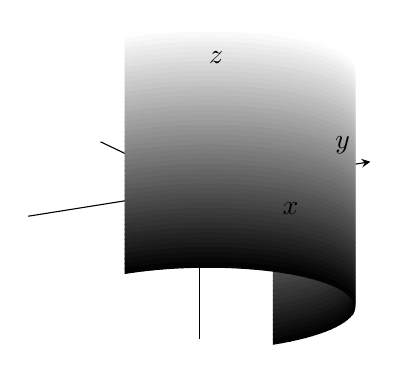
\begin{tikzpicture}
            \begin{axis}[
                view={60}{20},
                axis lines=middle,
                xlabel={$x$}, ylabel={$y$}, zlabel={$z$},
                xmin=-4, xmax=4, ymin=-2.5, ymax=2.5, zmin=-2.5, zmax=2.5,
                ticks=none
            ]
            \addplot3[
                samples=50,
                domain=0:pi,
                y domain=-2:2,
                surf,
                shader=flat,
                colormap/blackwhite
            ]
            (
                {3 * cos(deg(x))},
                {2 * sin(deg(x))},
                {y}
            );
            \end{axis}
            \end{tikzpicture}
    \end{center}

    \item[(b)] Given parameterization:
    \[ \vec{r}(u, v) = \langle u \sin v, u^2, u \cos v \rangle, \quad 0 \leq u \leq 3, \quad 0 \leq v \leq 2\pi \]

    \[ x(u, v) = u \sin v, \quad y(u, v) = u^2, \quad z(u, v) = u \cos v \]

    \[  \sin v = \frac{x}{u}, \quad \cos v = \frac{z}{u} \]

    \[ \left( \frac{x}{u} \right)^2 + \left( \frac{z}{u} \right)^2 = 1 \]

    \[ x^2 + z^2 = u^2 \]

    \[ x^2 + z^2 = y \]

    \begin{center}
        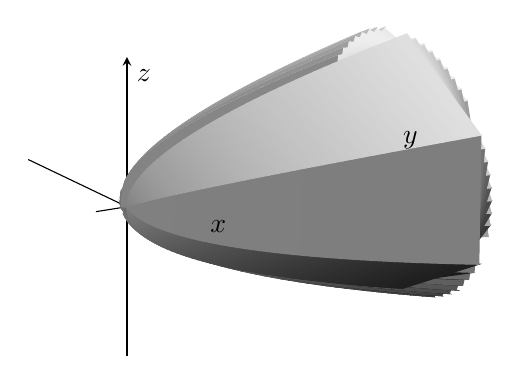
\begin{tikzpicture}
            \begin{axis}[
                view={60}{20},
                axis lines=middle,
                xlabel={$x$}, ylabel={$y$}, zlabel={$z$},
                xmin=-3.5, xmax=3.5, ymin=-1, ymax=10, zmin=-3.5, zmax=3.5,
                ticks=none
            ]
            \addplot3[
                samples=50,
                domain=0:3,
                y domain=0:360,
                surf,
                shader=flat,
                colormap/blackwhite
            ]
            (
                {x * sin(deg(y))},
                {x^2},
                {x * cos(deg(y))}
            );
            \end{axis}
            \end{tikzpicture}
    \end{center}

\end{enumerate}




\qs{}{
    Consider the surface \( S \) described by \( x - 4y^2 - z^2 + 3 = 0 \).
    \begin{enumerate}
        \item[(a)] Find a parametrization of \( S \) of the form \( \vec{r}_1(u, v) = \langle f(u, v), u, v \rangle \). Give the domain for your parametrization.
        \item[(b)] Find a parametrization of \( S \) of the form \( \vec{r}_2(u, v) = \langle v, f(v) \cos u, g(v) \sin u \rangle \). Give the domain for your parametrization.
        \item[(c)] How must we restrict the parameters \( (u, v) \) in part (a) if we only want the part of \( S \) that lies in front of the \( yz \)-plane, i.e., where \( x \geq 0 \)?
        \item[(d)] How must we restrict the parameters \( (u, v) \) in part (b) if we only want the part of \( S \) that lies in front of the \( yz \)-plane?
    \end{enumerate}
}


\begin{enumerate}
    \item[(a)]
    \[ x = 4y^2 + z^2 - 3. \]    
    \[ \vec{r}_1(u, v) = \langle 4u^2 + v^2 - 3, u, v \rangle. \]    
    \[ (u, v) \in \mathbb{R}^2. \]
    
    \item[(b)] 
    \[ \vec{r}_2(u, v) = \langle v, f(v) \cos u, g(v) \sin u \rangle \] 
    \[ x = v \quad  y = f(v) \cos u \quad  z = g(v) \sin u \] 
    \[ v - 4\left[f(v) \cos u\right]^2 - \left[g(v) \sin u\right]^2 + 3 = 0. \]
    \[ v - 4f(v)^2 \cos^2 u - g(v)^2 \sin^2 u + 3 = 0. \]
    \[ 4f(v)^2 = k \quad \text{and} \quad g(v)^2 = k \]
    \[ k = v + 3 \]
    \[ f(v) = \frac{1}{2} \sqrt{v + 3}, \quad g(v) = \sqrt{v + 3}. \]    
    \[ \vec{r}_2(u, v) = \left\langle v, \frac{1}{2} \sqrt{v + 3} \cos u, \sqrt{v + 3} \sin u \right\rangle \]    
    \[ v \geq -3, \quad u \in \mathbb{R} \]
    
    \item[(c)] 
    
    \[ x = 4u^2 + v^2 - 3 \geq 0 \]    
    \[ 4u^2 + v^2 \geq 3 \]
        
    \item[(d)] 
    \[ v \geq 0. \]
        
    \[ v \geq 0, \quad u \in \mathbb{R} \]
\end{enumerate}


\newpage 

\qs{}{
    Find parametric equations for each of the following surfaces.
    \begin{enumerate}
        \item[(a)] The part of the plane \( z = x + 3 \) that lies inside the cylinder \( x^2 + y^2 = 1 \).
        \item[(b)] The surface obtained by rotating the curve \( x = 4y^2 - y^4 \), \( -2 \leq y \leq 2 \) about the \( y \)-axis.
        \item[(c)] The ellipsoid \( \frac{x^2}{4} + 4y^2 + \frac{z^2}{9} = 1 \).
    \end{enumerate}
}

    a)

    \[ x = r \cos\theta, \quad y = r \sin\theta, \]
    \[ r \in [0, 1] \quad  \text{and} \theta \in [0, 2\pi) \]

    \[ z = r \cos\theta + 3. \]

    \[ \begin{cases}
    x = r \cos\theta, \\
    y = r \sin\theta, \\
    z = r \cos\theta + 3,
    \end{cases} \]
    \[ 0 \leq r \leq 1 \quad  \text{and} \quad  0 \leq \theta < 2\pi \].

    b)
    \[ \begin{cases}
    x = \left(4y^2 - y^4\right) \cos\theta, \\
    y = y, \\
    z = \left(4y^2 - y^4\right) \sin\theta,
    \end{cases} \]
    \[ -2 \leq y \leq 2 \quad \text{and} \quad 0 \leq \theta < 2\pi \].


    c)

    \[ X = \dfrac{x}{2}, \quad Y = 2y, \quad Z = \dfrac{z}{3} \]
    \[ X^2 + Y^2 + Z^2 = 1 \]

    \[ \begin{cases}
    X = \sin\phi \cos\theta, \\
    Y = \sin\phi \sin\theta, \\
    Z = \cos\phi,
    \end{cases} \]
    \[ \phi \in [0, \pi] \quad \text{and} \quad  \theta \in [0, 2\pi) \]

    \[ \begin{cases}
    x = 2X = 2\sin\phi \cos\theta, \\
    y = \dfrac{Y}{2} = \dfrac{1}{2}\sin\phi \sin\theta, \\
    z = 3Z = 3\cos\phi.
    \end{cases} \]

    \[
    \begin{cases}
    x = 2 \sin\phi \cos\theta, \\
    y = \dfrac{1}{2} \sin\phi \sin\theta, \\
    z = 3 \cos\phi,
    \end{cases} \]
    \[ 0 \leq \phi \leq \pi \quad \text{and} \quad 0 \leq \theta < 2\pi \] 



\qs{}{
    Find the tangent plane to the parametric surface \( \vec{r}(u, v) = \langle u \sin v, u^2, u \cos v \rangle \) at the point where \( u = 1 \) and \( v = \frac{\pi}{3} \). Write the plane both in the vector form \( \vec{r}(u, v) = \vec{r}_0 + u \vec{a} + v \vec{b} \) and in the form \( ax + by + cz = d \).
}

\sol{
    \[ \vec{r}_0 = \vec{r}(1, \tfrac{\pi}{3}) = \left\langle 1 \cdot \sin \tfrac{\pi}{3},\ 1^2,\ 1 \cdot \cos \tfrac{\pi}{3} \right\rangle = \left\langle \tfrac{\sqrt{3}}{2},\ 1,\ \tfrac{1}{2} \right\rangle. \]
    \[ \vec{r}_u(u, v) = \left\langle \sin v,\ 2u,\ \cos v \right\rangle \]
    \[ \vec{r}_v(u, v) = \left\langle u \cos v,\ 0,\ -u \sin v \right\rangle \]
    \[ \vec{r}_u(1, \tfrac{\pi}{3}) = \left\langle \sin \tfrac{\pi}{3},\ 2,\ \cos \tfrac{\pi}{3} \right\rangle = \left\langle \tfrac{\sqrt{3}}{2},\ 2,\ \tfrac{1}{2} \right\rangle, \]
    \[ \vec{r}_v(1, \tfrac{\pi}{3}) = \left\langle 1 \cdot \cos \tfrac{\pi}{3},\ 0,\ -1 \cdot \sin \tfrac{\pi}{3} \right\rangle = \left\langle \tfrac{1}{2},\ 0,\ -\tfrac{\sqrt{3}}{2} \right\rangle. \]
    \[ \vec{r}(s, t) = \vec{r}_0 + s\,\vec{r}_u(1, \tfrac{\pi}{3}) + t\,\vec{r}_v(1, \tfrac{\pi}{3}) \]
    \[ \vec{r}(s, t) = \left\langle \tfrac{\sqrt{3}}{2},\ 1,\ \tfrac{1}{2} \right\rangle + s \left\langle \tfrac{\sqrt{3}}{2},\ 2,\ \tfrac{1}{2} \right\rangle + t \left\langle \tfrac{1}{2},\ 0,\ -\tfrac{\sqrt{3}}{2} \right\rangle. \]
    \[ \vec{n} = \vec{r}_u(1, \tfrac{\pi}{3}) \times \vec{r}_v(1, \tfrac{\pi}{3}) = \begin{vmatrix}
    \mathbf{i} & \mathbf{j} & \mathbf{k} \\
    \tfrac{\sqrt{3}}{2} & 2 & \tfrac{1}{2} \\
    \tfrac{1}{2} & 0 & -\tfrac{\sqrt{3}}{2}
    \end{vmatrix}. \]
    \[ \vec{n} = \left( -\sqrt{3},\ 1,\ -1 \right) \]

    \[ \vec{n} \cdot (\vec{r} - \vec{r}_0) = 0. \]
    \[ -\sqrt{3}(x - \tfrac{\sqrt{3}}{2}) + 1(y - 1) - 1(z - \tfrac{1}{2}) = 0 \]
    \[ -\sqrt{3}x + y - z + \left( \tfrac{3}{2} - 1 + \tfrac{1}{2} \right) = 0, \]
    \[ -\sqrt{3}x + y - z + 1 = 0. \]
    \[ \sqrt{3}x - y + z = 1 \]
    \[ \sqrt{3}\,x\ -\ y\ +\ z\ =\ 1 \]
    \[ \vec{r}(s, t) = \left\langle \tfrac{\sqrt{3}}{2},\ 1,\ \tfrac{1}{2} \right\rangle + s \left\langle \tfrac{\sqrt{3}}{2},\ 2,\ \tfrac{1}{2} \right\rangle + t \left\langle \tfrac{1}{2},\ 0,\ -\tfrac{\sqrt{3}}{2} \right\rangle. \]
    \[ \sqrt{3}\,x\ -\ y\ +\ z\ =\ 1 \]}

\end{document}